Necesita un medio para propagarse. Debido a esto, no pueden propagarse en el vacío. Este tipo de onda puede ser \longitudinal\ o \transversal.

\begin{figure}[H]
  \centering
  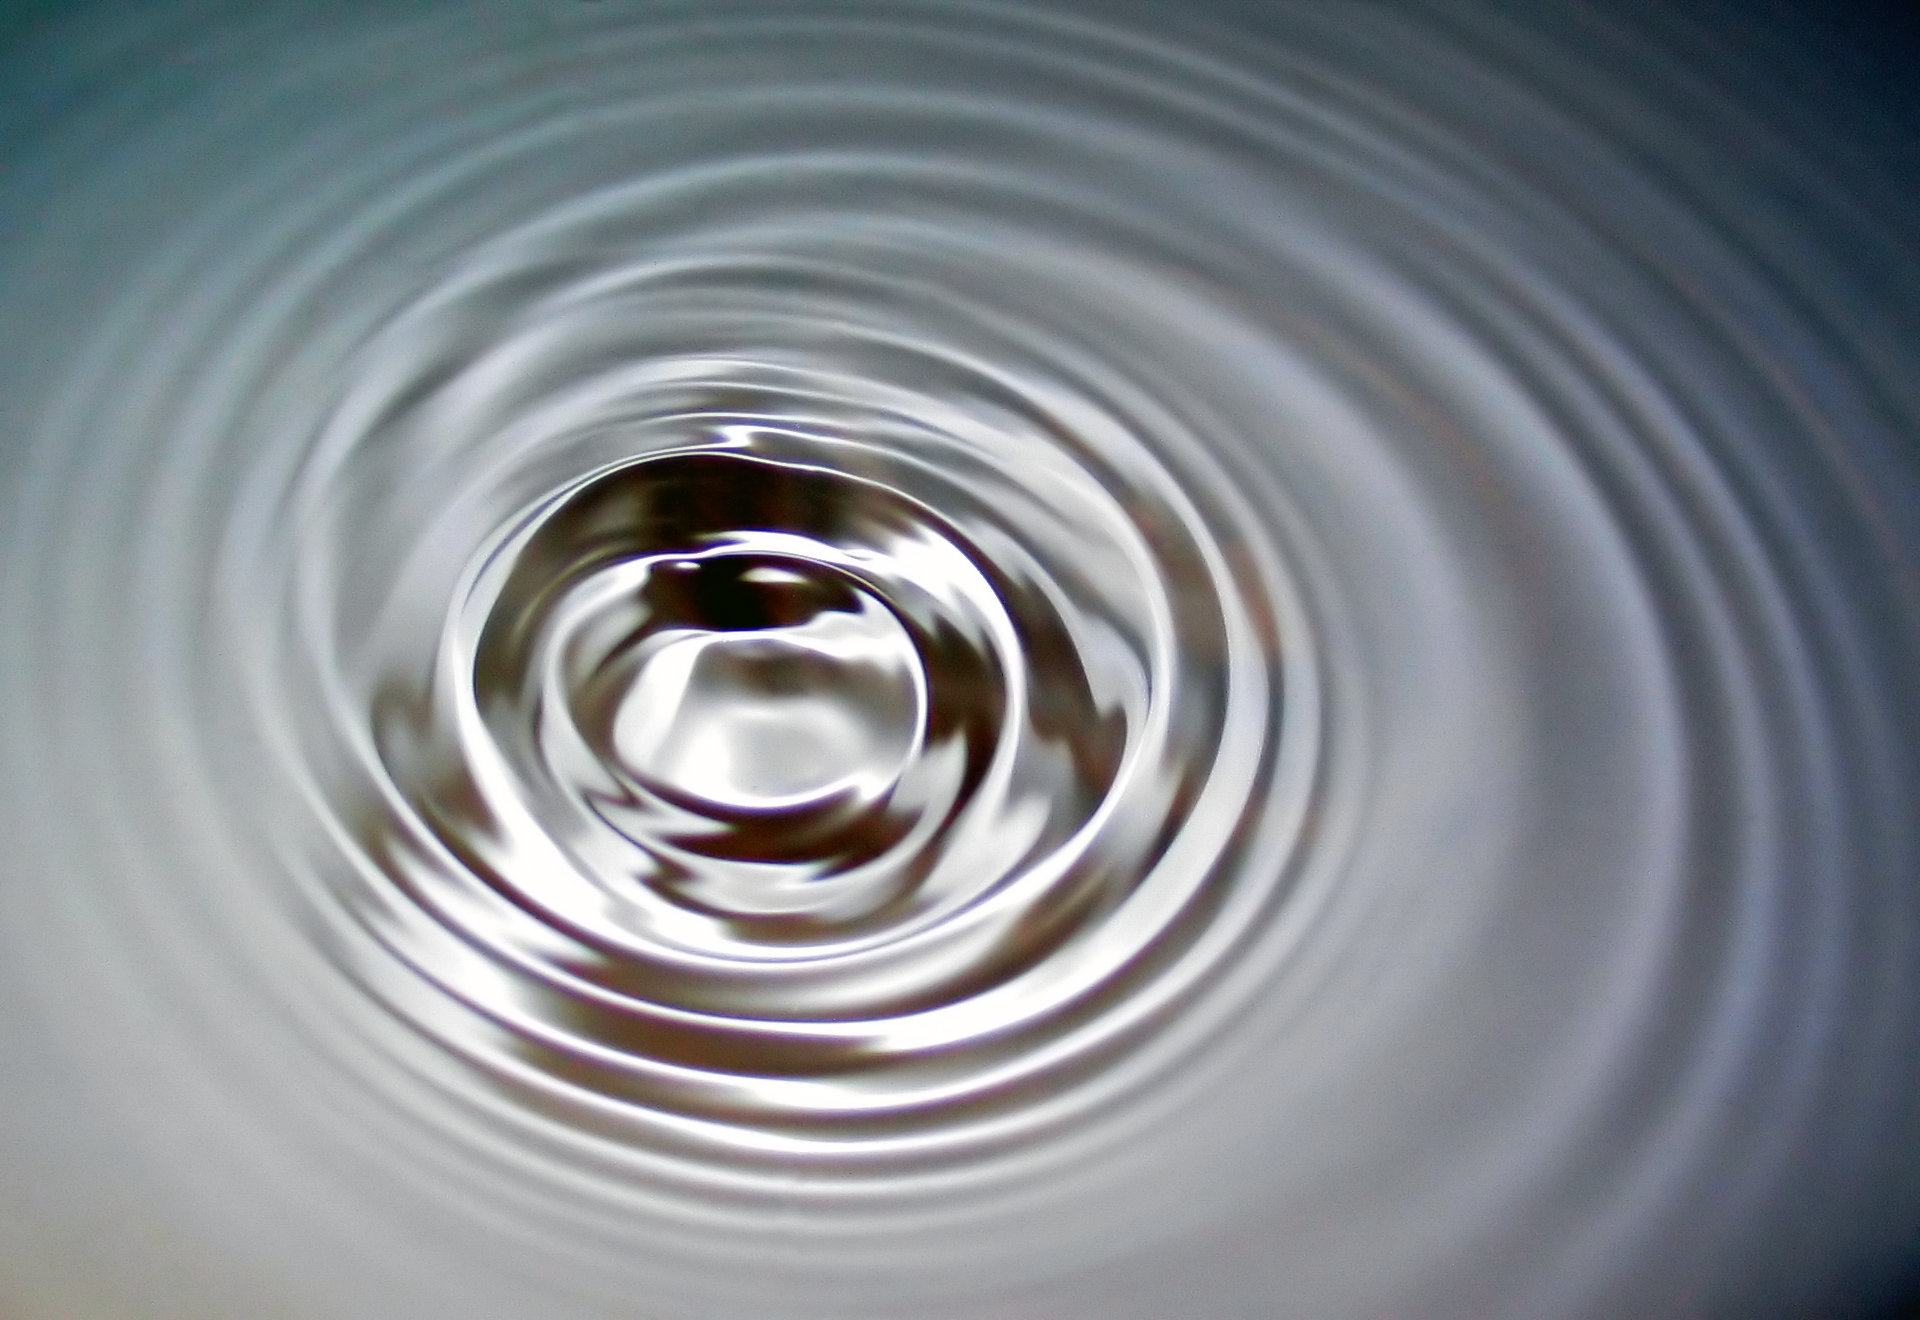
\includegraphics[scale=0.2]{imagenes/ondas_agua.png}
  \caption{Ondas en el agua\cite{wikiwaves}}
\end{figure}

Ejemplos:

\begin{itemize}
  \item Sonido.
  \item Ondas en el agua.
  \item Ondas sísmicas.
  \item Ondas en la cuerda de un instrumento musical.
  \item Ondas en resortes.
\end{itemize}
